% Created 2023-11-28 Tue 13:47
% Intended LaTeX compiler: pdflatex




\documentclass[presentation, smaller]{beamer}
\usepackage[utf8]{inputenc}
\usepackage[T1]{fontenc}
\usepackage{graphicx}
\usepackage{longtable}
\usepackage{wrapfig}
\usepackage{rotating}
\usepackage[normalem]{ulem}
\usepackage{amsmath}
\usepackage{amssymb}
\usepackage{capt-of}
\usepackage{hyperref}
\usepackage{amsmath,amssymb}
\usetheme[]{default}
\usepackage{tikz}
\usetikzlibrary[topaths] \newcount\mycount
\usepackage{pgf}

\pgfmathsetseed{\number\pdfrandomseed} % to ensure that it is randomized
% use \randomseed for xelatex

\newcommand{\thecmd}[1]{%
\pgfmathsetmacro{\thenum}{int(random(ceil(#1-#1/4),floor(#1+#1/4)))}%
\thenum%
}%
\usepackage{xcolor}
\usepackage{framed}
\usepackage{amsthm}
\usepackage[utf8]{inputenc}

\colorlet{shadecolor}{CoalGray!15}

\newcommand{\propnumber}{} % initialize
\newtheorem*{prop}{Proposition \propnumber}
\newenvironment{propc}[1]
{\renewcommand{\propnumber}{#1}%
\begin{prop}}
{\end{prop}}
\frenchspacing
\usetheme{purduegold}
\author{John Biechele-Speziale, Kushagra Kapoor, Jae Heo}
\date{\today}
\title{POMDPs: Myths, Legends, and Reality}
\hypersetup{
 pdfauthor={John Biechele-Speziale, Kushagra Kapoor, Jae Heo},
 pdftitle={POMDPs: Myths, Legends, and Reality},
 pdfkeywords={},
 pdfsubject={},
 pdfcreator={Emacs 28.1 (Org mode 9.6.1)}, 
 pdflang={English}}
\begin{document}

\maketitle
\begin{frame}{Outline}
\setcounter{tocdepth}{1}
\tableofcontents
\end{frame}

\setbeamertemplate{footline}[frame number]

\section{POMDP Variants and Applications}

\begin{frame}{Model-Based Approaches: Value Iteration}
    \begin{itemize}
        \item Value Iteration for an observable discrete MDP:
        \begin{itemize}
            \item One entry per state: $V(s_1) = 0.9$
        \end{itemize}
        
        \item For a 2 state POMDP, the belief state looks like : $[0.25, 0.75]$. 
        \begin{itemize}
            \item Belief space is continuous $\implies$ No longer one entry per state.
        \end{itemize}
        \item Problem: Continuous MDP
        \begin{itemize}
            \item key insight is that the finite horizon value function is piecewise linear and convex (PWLC) for every horizon length
        \end{itemize}
        
    \end{itemize}
    
\end{frame}

\begin{frame}{Model-Based Approaches: Value Iteration}
    \begin{itemize}
     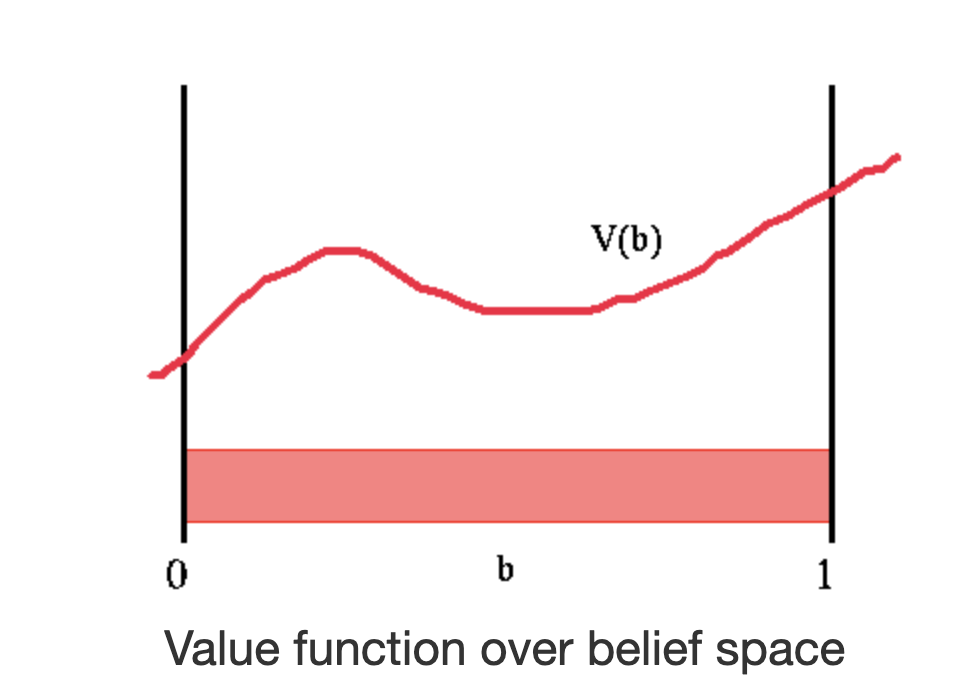
\includegraphics[scale = 0.3]{pic_1.png}
    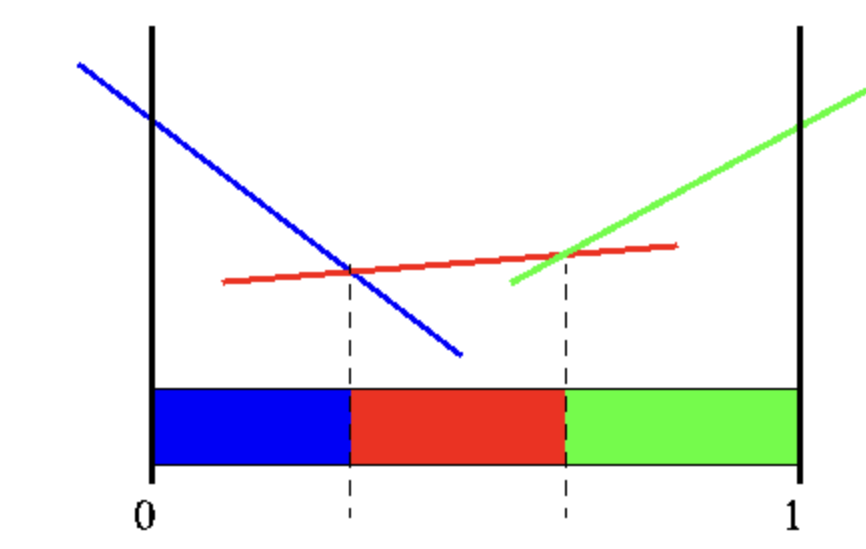
\includegraphics[scale = 0.32]{pic_3.png}
    \end{itemize}
    
\end{frame}

\begin{frame}{Model-based Approaches: Value Iteration Algorithms}
  \textbf{Monahan’s Enumeration Algorithm:}
  \begin{itemize}
    \item Calculates all possible ways HPOMDPVn could be constructed.
    \item Exploits the known structure of the value function.
    \item Generates a finite number of vectors in each HPOMDPVn.
  \end{itemize}

  \textbf{Incremental Pruning:}
  \begin{itemize}
    \item Saves computation time by pruning dominated vectors incrementally.
    \item Utilizes the property: $prune(G⊕G'⊕G'') = prune(prune(G⊕G')⊕G'')$.
    \item Leads to better performance with a slow growth of constraints in the linear program.
  \end{itemize}
\end{frame}

\begin{frame}{Model-based Approaches: Point-based Value Iteration Methods}
  \textbf{Approximate Solutions:}
  \begin{itemize}
    \item Focuses on computing solutions for reachable parts of the belief simplex.
    \item Uses a sampled set of belief points for planning.
    \item Allows planning on a limited set of prototype beliefs, making it tractable for large state spaces.
  \end{itemize}
\end{frame}


\begin{frame}{Approximate Methods}
  \textbf{Grid-based Approaches:}
  \begin{itemize}
    \item Sidesteps intractability with fixed or variable grid on the belief simplex.
    \item Performs value backups, preserving only grid point values.
    \item Interpolates non-grid point values.
  \end{itemize}

  \textbf{Policy Search:}
  \begin{itemize}
    \item Searches for a good policy within a restricted class.
    \item Options include gradient ascent, stochastic local search, and methods like PEGASUS.
    \item Demonstrates success but challenging with potential local optima.
  \end{itemize}

  \textbf{Heuristic Search:}
  \begin{itemize}
    \item Builds a tree over (a,o) pairs from an initial belief node.
    \item Uses branch-and-bound for upper and lower bounds on returns.
    \item Provides an alternative approach for solving POMDPs.
  \end{itemize}
\end{frame}



\begin{frame}{Model-free Approaches}
  \textbf{Challenges Without Models:}
  \begin{itemize}
    \item When no models are available, model-based methods face challenges.
    \item QMDP requires knowledge of the complete POMDP model.
  \end{itemize}

  \textbf{Direct and Indirect Reinforcement Learning:}
  \begin{itemize}
    \item Two ways of tackling decision-making without a priori models.
    \item Direct methods map observation histories directly to actions.
    \item Indirect methods attempt to reconstruct the POMDP model by interacting with it.
  \end{itemize}
\end{frame}




\begin{frame}[label={sec:org9887ed5}]{References}
\nocite{*}
\bibliographystyle{ieeetr}
\bibliography{ref}
\end{frame}
\end{document}
